\subsection{Pruebas Unitarias de las Reglas de Seguridad de Firestore}\label{subsec:pruebas-reglas-firestore}

El control de acceso a los datos en Paralegales se delega en las Reglas de Seguridad de Firestore, una capa declarativa que decide, para cada operación de lectura, escritura o eliminación, si la solicitud está autorizada en función de la identidad del usuario y del estado de los datos. Por ser la última línea de defensa frente a accesos indebidos, su corrección se valida mediante una \textit{suite} de pruebas unitarias automatizada y repetible.

\subsubsection{Entorno de ejecución y herramientas}

La \textit{suite} se construye con Vitest y la librería oficial \texttt{@firebase/rules-unit-testing}, y se ejecuta contra la \textit{Firebase Emulator Suite}, que despliega de forma local y efímera una instancia de Firestore sin incurrir en costos ni afectar entornos reales. La gestión del entorno se centraliza en dos utilidades: una de inicialización, que carga las reglas reales del archivo \texttt{firestore.rules} —de modo que se verifica exactamente el artefacto que se despliega—, siembra opcionalmente datos de partida con las reglas deshabilitadas y expone un contexto de ejecución \textbf{autenticado} o \textbf{no autenticado}; y otra que limpia los datos y libera el entorno tras cada caso, garantizando el aislamiento. Sobre Vitest se definieron además dos \textit{matchers} personalizados, \texttt{toAllow} y \texttt{toDeny} —apoyados en \texttt{assertSucceeds} y \texttt{assertFails}—, que permiten redactar aserciones legibles del tipo \textit{``el propietario puede leer su documento''} o \textit{``un usuario no puede leer el de otro''}.

\subsubsection{Diseño de casos: pruebas positivas y negativas}

La \textit{suite} se organiza por colección y, dentro de cada una, por tipo de operación, combinando casos positivos y negativos para certificar tanto que el acceso legítimo funciona como que el indebido se bloquea. Las baterías cubren las colecciones críticas del dominio: las \textbf{reglas básicas} (rechazo de lecturas sobre colecciones no autorizadas o de eliminaciones no contempladas), la colección \texttt{users} (aislamiento entre usuarios: cada uno solo lee y crea su propio documento), la colección \texttt{payments} (solo el propietario accede a sus pagos, y las actualizaciones de los flujos de proceso se rechazan ante un solicitante no propietario o datos inválidos) y la colección \texttt{associations} (reglas de listado según el estado de autenticación). La predominancia de casos negativos —solicitudes que \textit{deben} fallar— es deliberada: confirmar que el acceso indebido se bloquea es justo el tipo de regresión que una validación manual pasa por alto.

\subsubsection{Ejecución}

La \textit{suite} se ejecuta mediante el \textit{script} \texttt{test:rules}, que levanta el emulador de Firestore y corre las pruebas en su contexto con \texttt{firebase emulators:exec}. De este modo, cada ejecución parte de un entorno limpio y aislado, con resultados deterministas y reproducibles. La \autoref{fig:pruebas-rules-run} muestra una corrida de la \textit{suite}.

\newcommand\pruebasRulesRunCaption{Ejecución de la \textit{suite} de pruebas unitarias de las reglas de seguridad de Firestore sobre la \textit{Firebase Emulator Suite}. \hspace{1em}}
\begin{figure}[H]
  \centering
  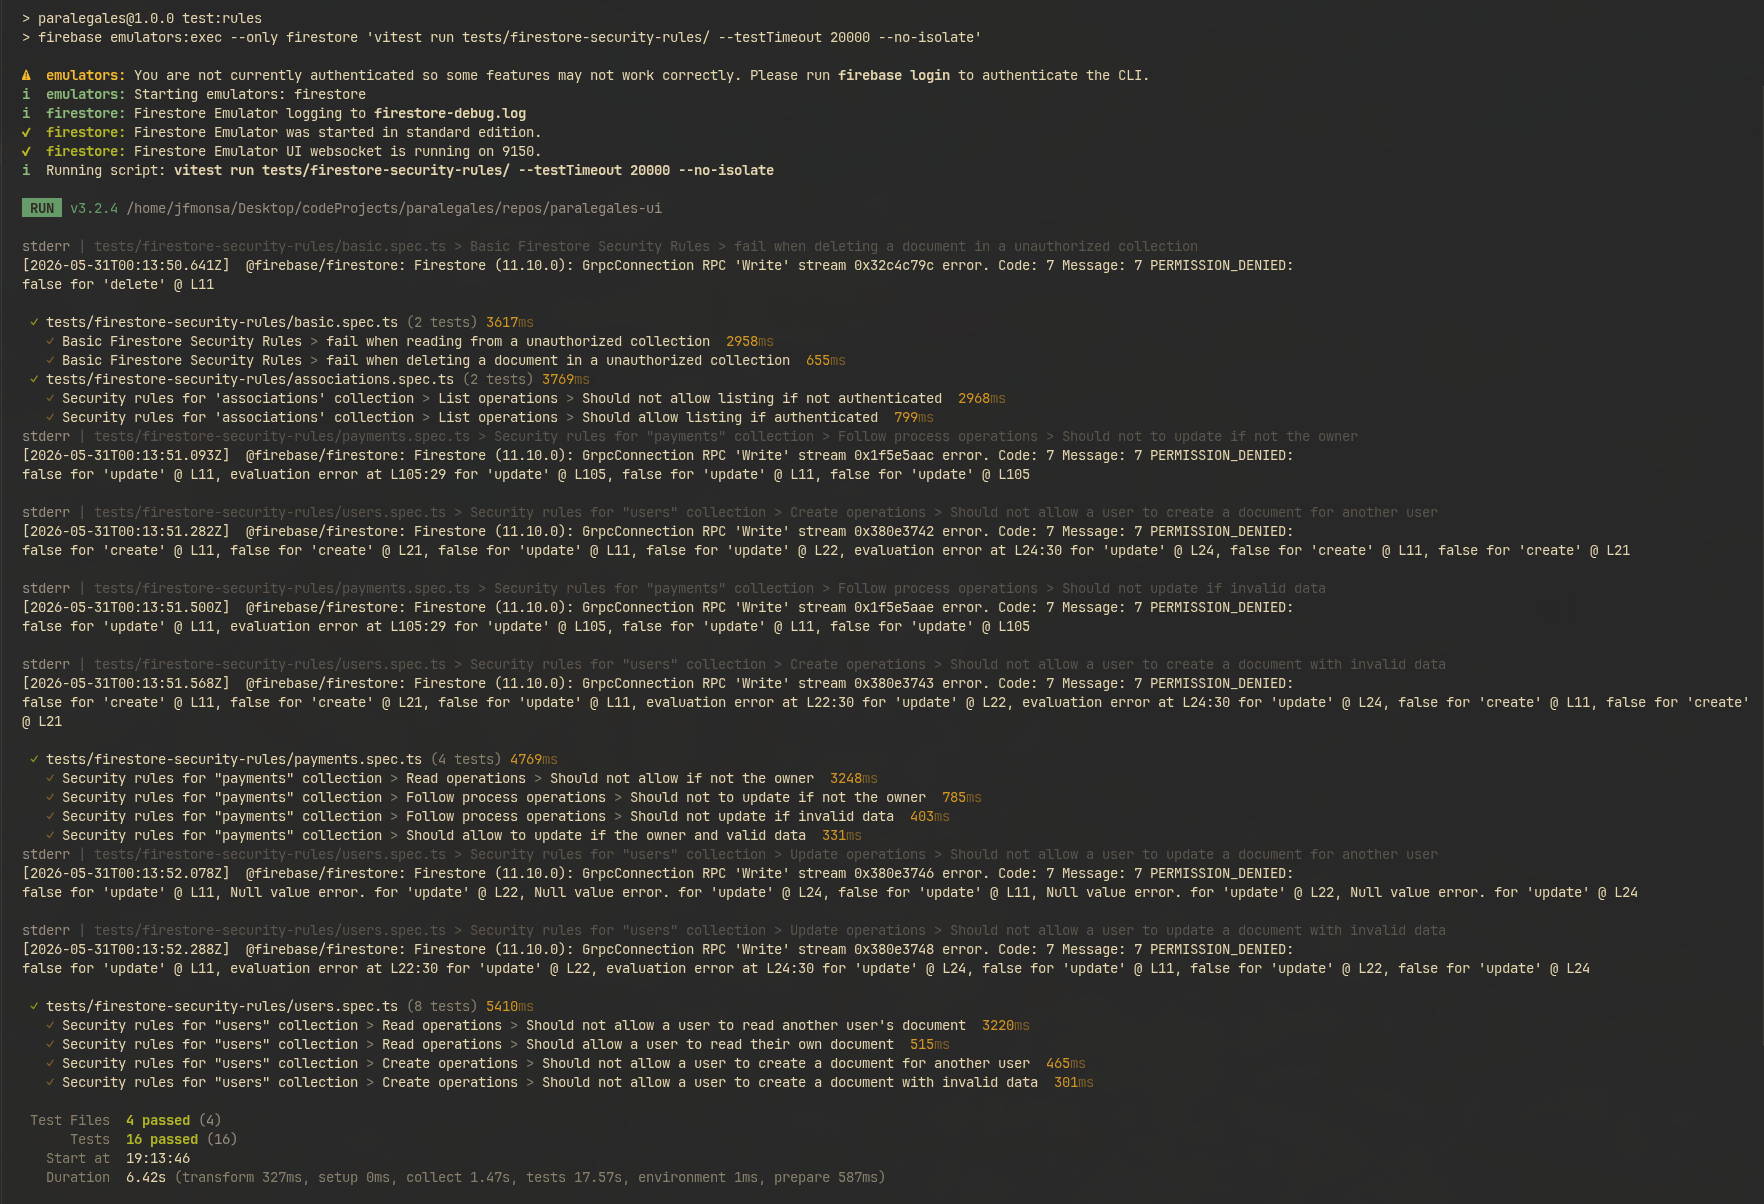
\includegraphics[width=1\textwidth]{img/figures/fig40-pruebas-rules-run.png}
  \caption[\pruebasRulesRunCaption]{\pruebasRulesRunCaption Fuente: Elaboración propia.}
  \label{fig:pruebas-rules-run}
\end{figure}
